\documentclass[aspectratio=169]{beamer}
\usepackage[utf8]{inputenc}
\usepackage{amsmath}
\usepackage{amsfonts}
\usepackage{amssymb}
\usepackage{graphicx}
\usepackage{booktabs}
\usepackage{multirow}
\usepackage{xcolor}
\usepackage{tikz}
\usepackage{pgfplots}
\usepackage{subcaption}
\usepackage{hyperref}

\usetheme{Madrid}
\usecolortheme{default}

% Custom colors
\definecolor{mscdark}{RGB}{0,51,102}
\definecolor{msclight}{RGB}{51,102,153}
\definecolor{mscaccent}{RGB}{204,102,0}

\setbeamercolor{title}{fg=mscdark}
\setbeamercolor{frametitle}{fg=mscdark}
\setbeamercolor{structure}{fg=msclight}

\title[LLM Performance in Taboo Games]{Evaluating Large Language Model Performance in Taboo Word Games: A Comprehensive Multi-Dimensional Analysis}
\subtitle{MSc Computer Science - Research Presentation}
\author{Your Name}
\institute{University Name}
\date{\today}

\begin{document}

% Title slide
\begin{frame}
\titlepage
\end{frame}

% Table of contents
\begin{frame}{Outline}
\tableofcontents
\end{frame}

\section{Introduction \& Background}

\begin{frame}{Research Context}
\begin{block}{Large Language Models \& Evaluation Challenges}
\begin{itemize}
    \item LLMs demonstrate remarkable capabilities in natural language understanding
    \item Traditional benchmarks often lack constraint-based evaluation
    \item Need for multi-dimensional assessment of communication abilities
    \item Taboo games provide natural framework for testing constraint satisfaction
\end{itemize}
\end{block}

\begin{block}{The Taboo Game Challenge}
\begin{itemize}
    \item \textbf{Objective}: Describe target words without using "taboo" words
    \item \textbf{Constraints}: Forbidden vocabulary, limited turns, multi-turn interaction
    \item \textbf{Skills Tested}: Semantic reasoning, constraint satisfaction, strategic communication
\end{itemize}
\end{block}

\begin{block}{Research Questions}
\begin{itemize}
    \item How do different LLMs perform under lexical constraints?
    \item What linguistic factors influence success in constrained language tasks?
    \item Which models excel at constraint-following vs. semantic understanding?
\end{itemize}
\end{block}
\end{frame}

\section{Literature Review}

\begin{frame}{Related Work}
\begin{block}{LLM Evaluation Evolution}
\begin{itemize}
    \item \textbf{Static Benchmarks}: MMLU (57 domains), AIME 2024, MATH-500, HumanEval
    \item \textbf{Interactive Evaluation}: LMSys Chatbot Arena (Elo rating), LiveCodeBench
    \item \textbf{Limitation}: Need for multi-dimensional, constraint-based evaluation
\end{itemize}
\end{block}

\begin{block}{Constrained Language Games}
\begin{itemize}
    \item \textbf{clembench Taboo}: Cooperative LLM dialogue evaluation
    \item \textbf{SPAG (Adversarial Taboo)}: Self-playing adversarial language games
    \item \textbf{Taboo Model Organism}: Knowledge extraction through constraint violation
    \item \textbf{Our Contribution}: Systematic multi-dimensional constraint satisfaction evaluation
\end{itemize}
\end{block}

\begin{block}{Evaluation Dimensions}
\begin{itemize}
    \item \textbf{Constraint Satisfaction}: Negative lexical constraints (taboo words)
    \item \textbf{Semantic Reasoning}: Indirect description and conceptual understanding
    \item \textbf{Strategic Communication}: Multi-turn adaptive interaction
\end{itemize}
\end{block}
\end{frame}

\section{Research Questions \& Objectives}

\begin{frame}{Project Objectives}
\begin{block}{Primary Aim}
Evaluate the reasoning and rule-following abilities of large language models using a constrained language benchmark inspired by the Taboo game.
\end{block}

\begin{block}{Five Core Objectives}
\begin{enumerate}
    \item Collect and label a dataset of target words and taboo words from WordNet
    \item Build a Taboo-style benchmark to test LLMs under constrained language conditions
    \item Create measurable scoring methods using regex, semantic similarity, and LLM-based judgment
    \item Test different LLMs (GPT-4, Claude, DeepSeek, Gemini) and compare performance
    \item Analyze results and draw conclusions about reasoning strengths and weaknesses
\end{enumerate}
\end{block}
\end{frame}

\section{Methodology}

\begin{frame}{Experimental Design Overview}
\begin{center}
\begin{figure}[h]
\centering
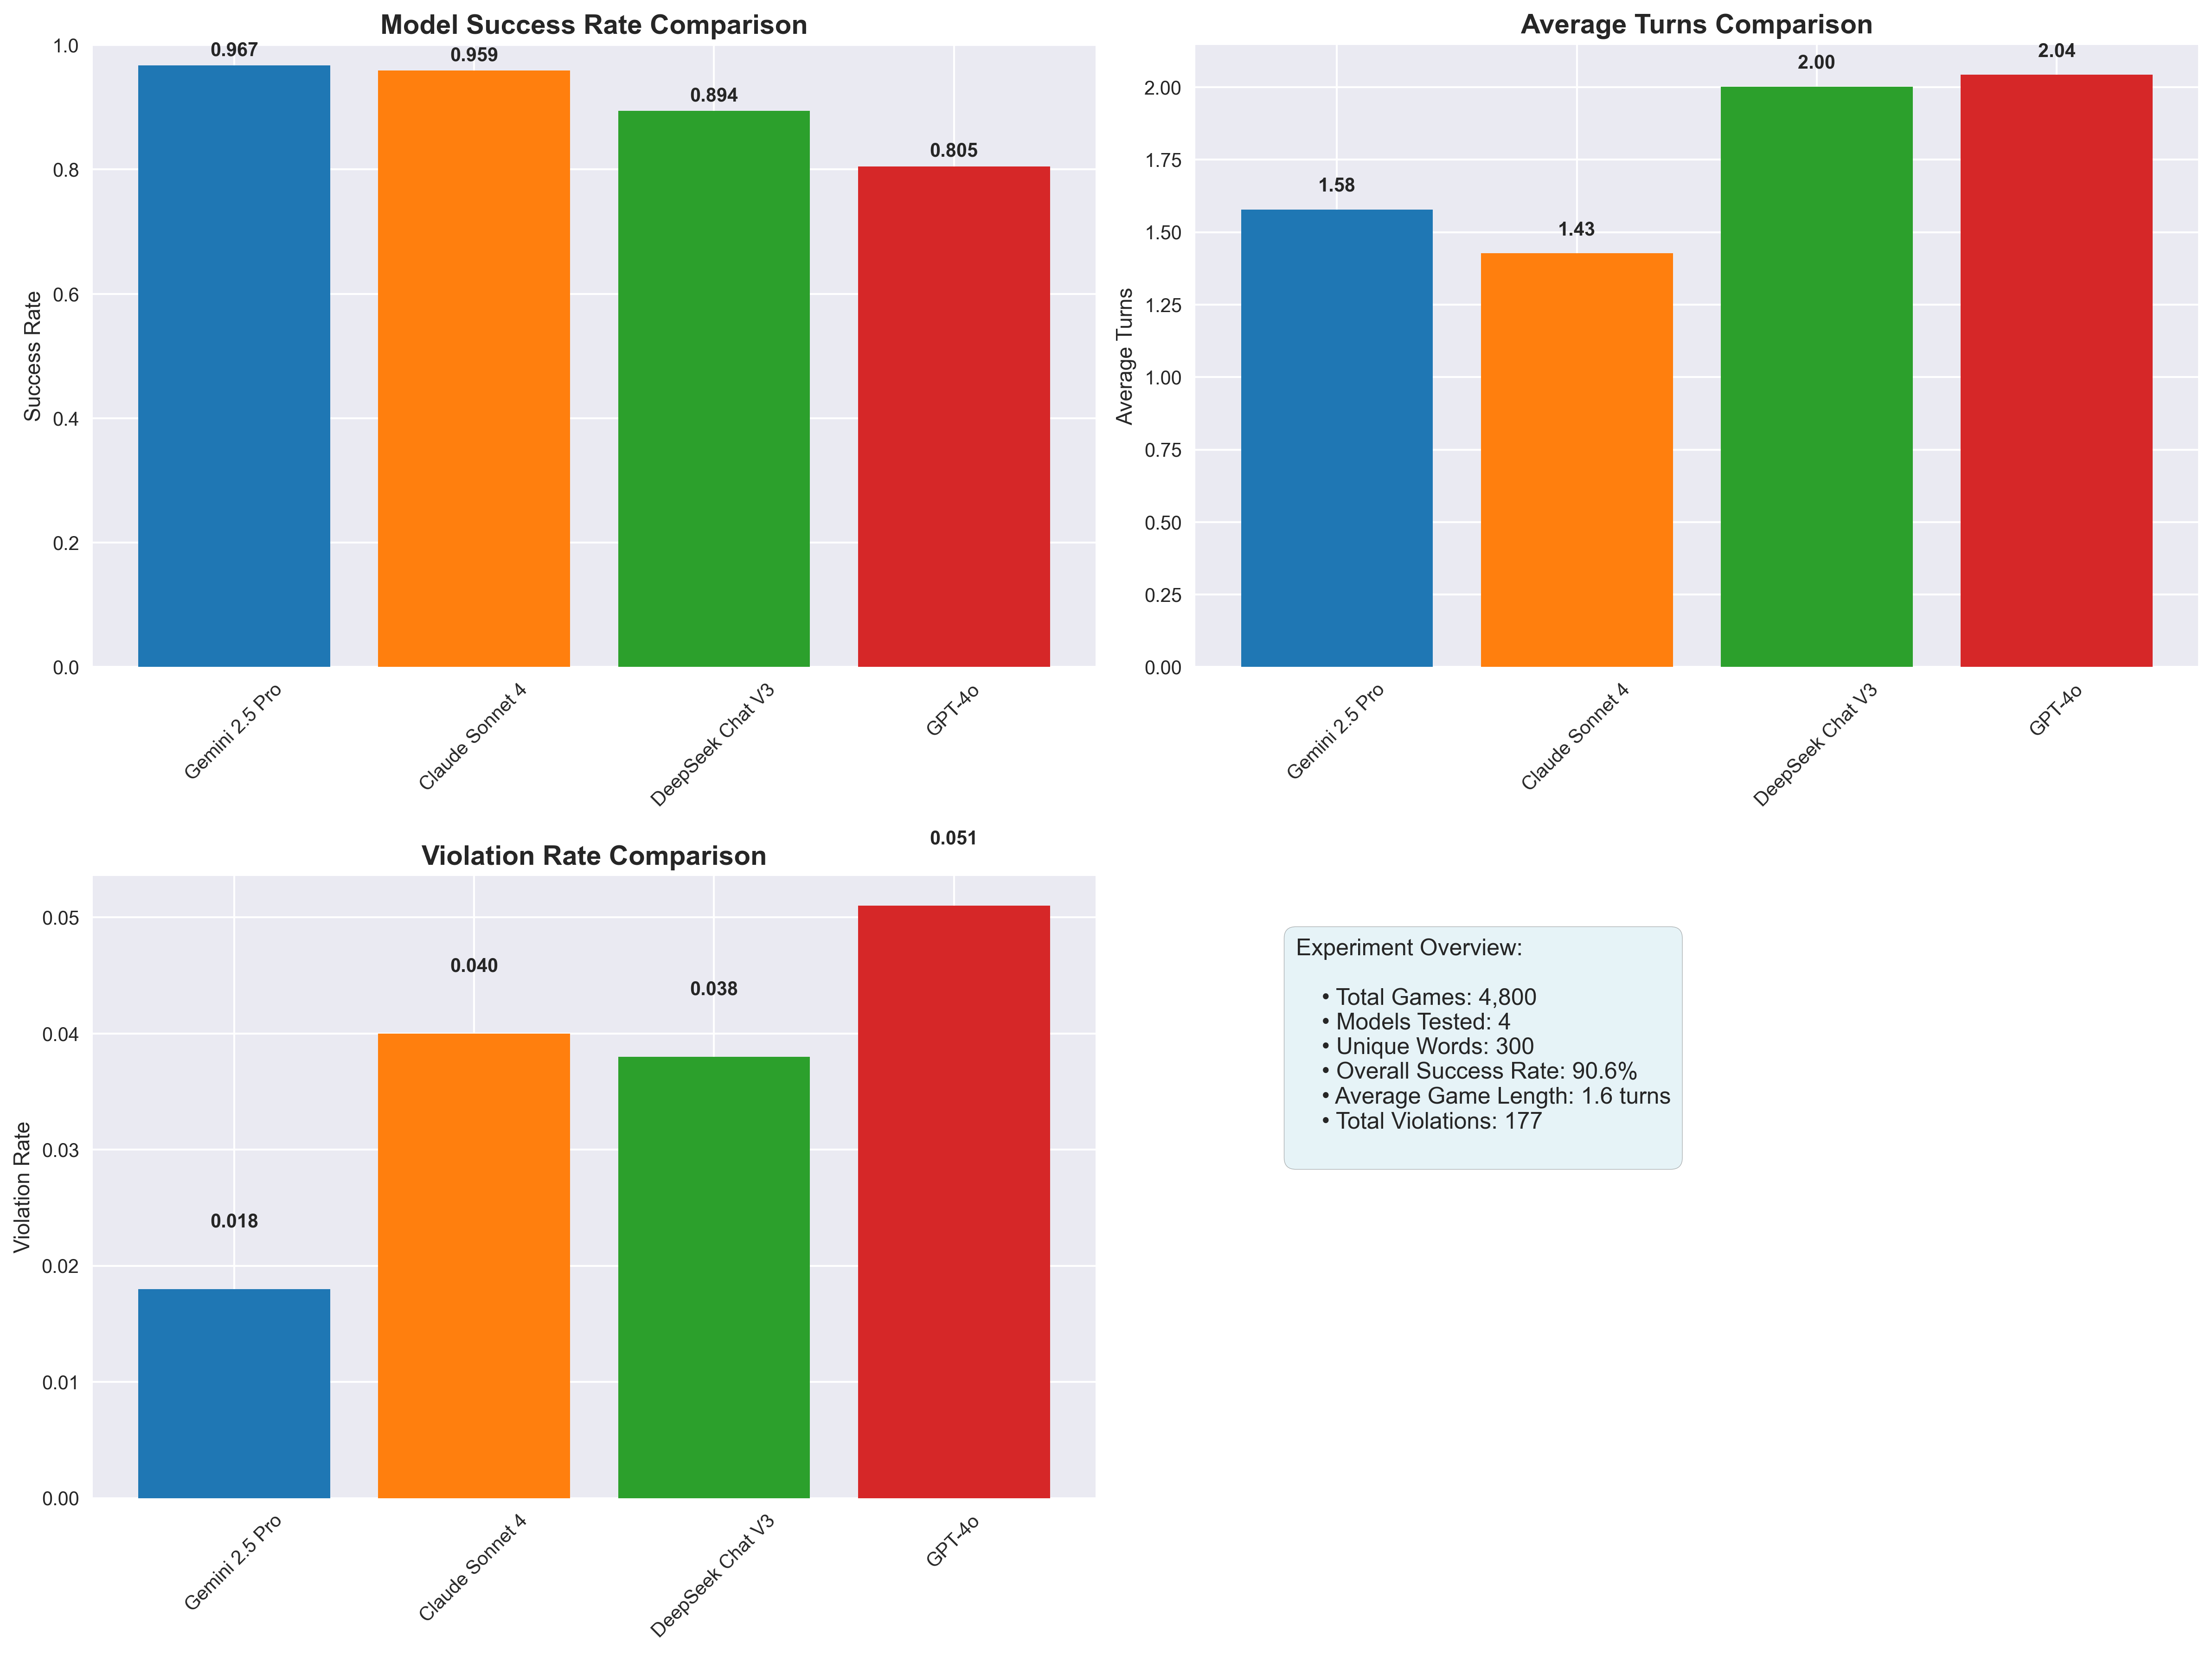
\includegraphics[width=0.9\textwidth]{comprehensive_figures/figure1_overview.png}
\end{figure}
\end{center}

\vspace{0.5cm}
\begin{columns}
\begin{column}{0.5\textwidth}
\begin{block}{Models Evaluated}
\begin{itemize}
    \item GPT-4o (OpenAI) - Upper bound
    \item Claude Sonnet 4 (Anthropic)
    \item Gemini 2.5 Pro (Google)
    \item DeepSeek Chat V3 (DeepSeek)
\end{itemize}
\end{block}
\end{column}

\begin{column}{0.5\textwidth}
\begin{block}{Scale}
\begin{itemize}
    \item \textbf{4,800 total games}
    \item \textbf{16 model pairs} (4×4)
    \item \textbf{300 words per pair}
\end{itemize}
\end{block}
\end{column}
\end{columns}
\end{frame}

\begin{frame}{Dataset Construction}
\begin{columns}
\begin{column}{0.6\textwidth}
\begin{block}{WordNet 3.1 Based Dataset}
\begin{itemize}
    \item \textbf{300 cards} across 5 domains
    \item \textbf{Domains}: General, Chemistry, CS, Finance, Philosophy
    \item \textbf{5 taboo words} per target (synonyms, hypernyms, etc.)
    \item Balanced domain distribution for analysis
\end{itemize}
\end{block}

\begin{block}{Game Configuration}
\begin{itemize}
    \item Maximum 5 turns per game
    \item Both hinter and guesser roles
    \item Strict taboo word violation detection
    \item Multi-turn adaptive interaction
\end{itemize}
\end{block}
\end{column}

\begin{column}{0.4\textwidth}
\begin{figure}[h]
\centering
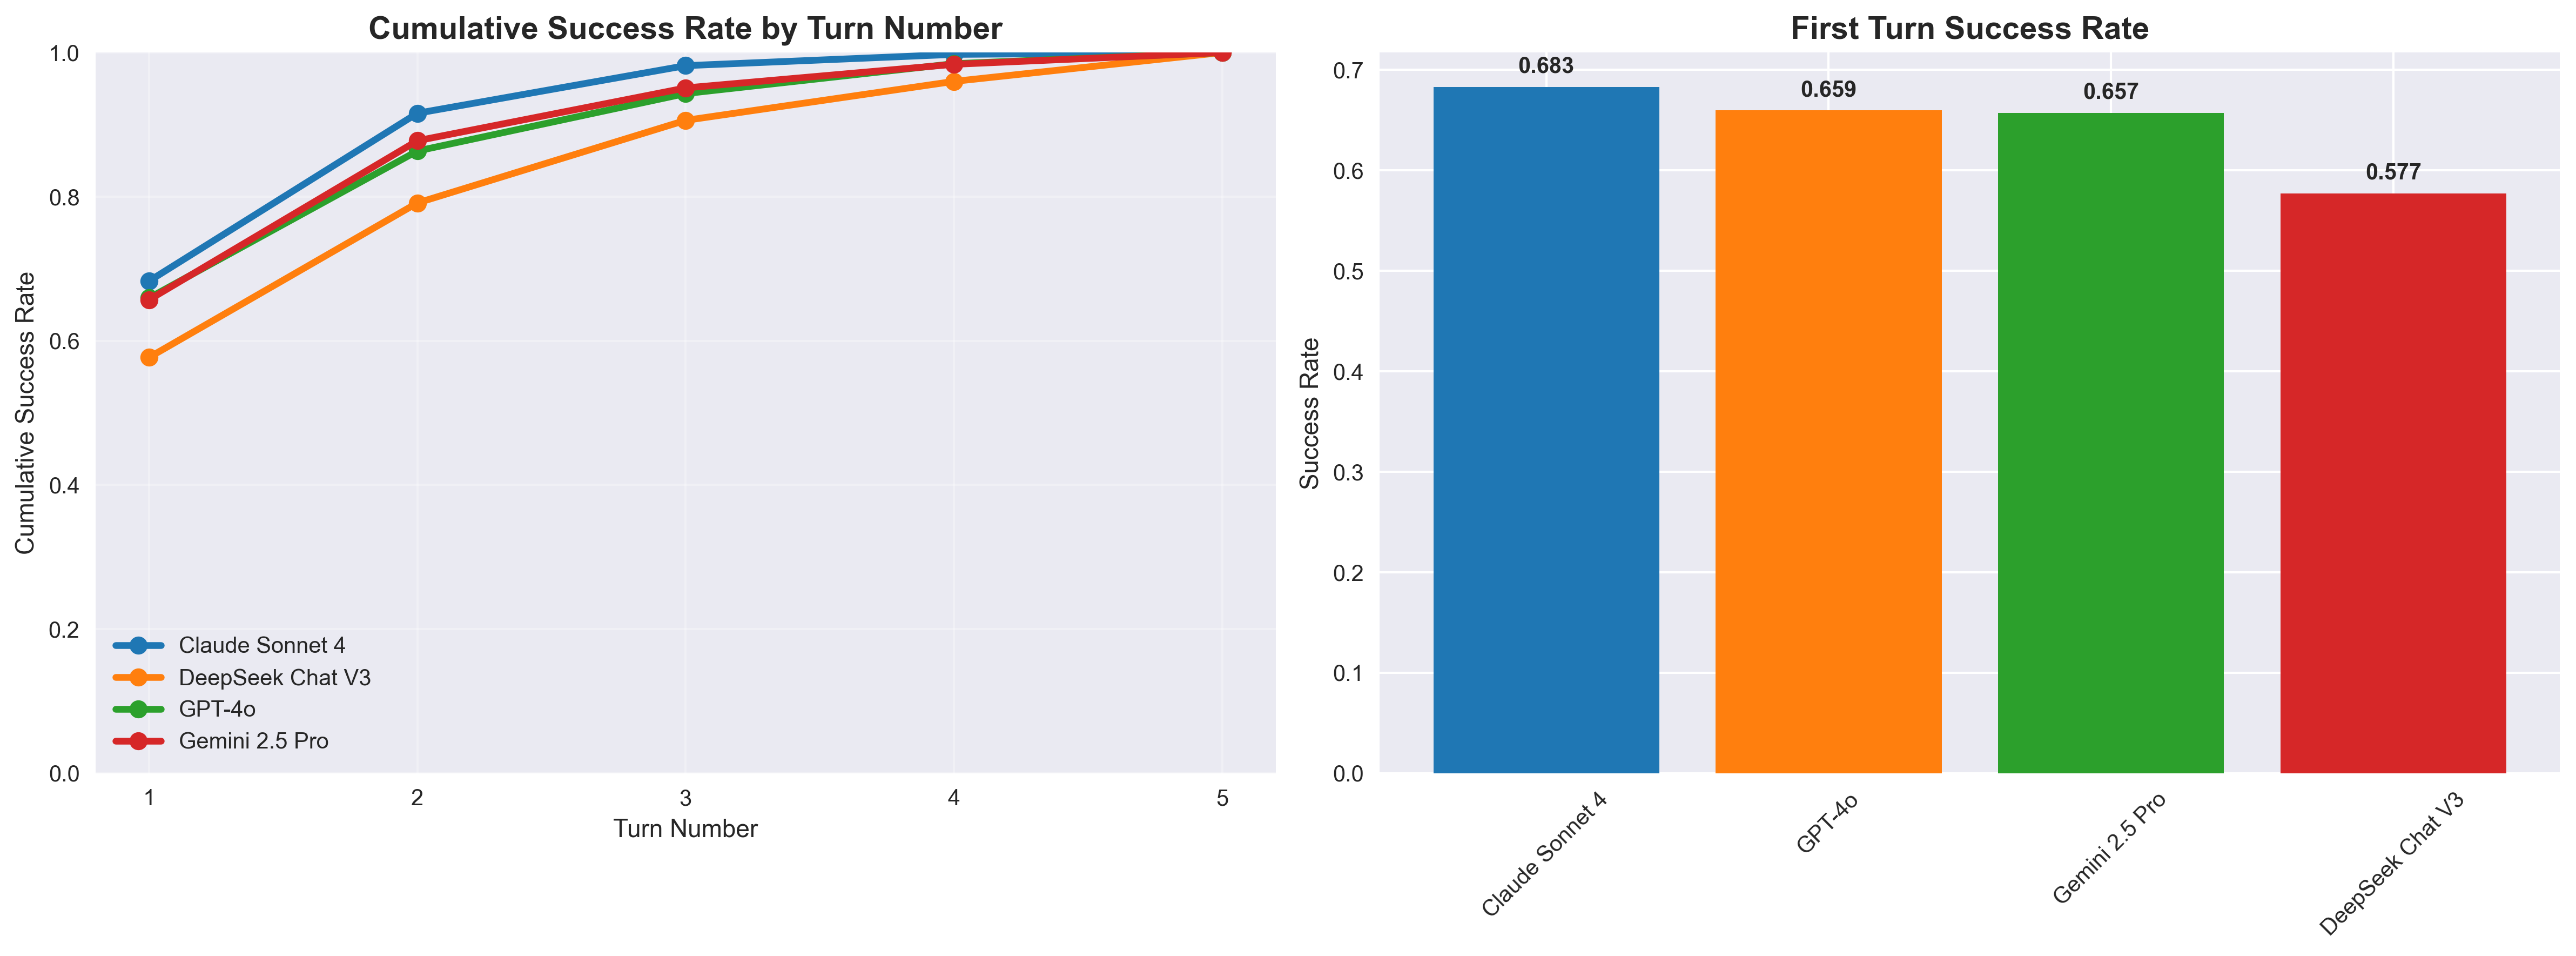
\includegraphics[width=0.95\textwidth]{comprehensive_figures/figure2_efficiency.png}
\caption{Turn Distribution}
\end{figure}
\end{column}
\end{columns}
\end{frame}

\begin{frame}{Evaluation Framework}
\begin{block}{Hinter (Clue Provider) Evaluation}
\begin{itemize}
    \item \textbf{Constraint Satisfaction}: Taboo word violation detection, format compliance
    \item \textbf{Semantic Quality}: Effectiveness of clues in guiding correct guesses
    \item \textbf{Efficiency}: Success rate within allowed turns
    \item \textbf{Rule Adherence}: Violation rate and compliance patterns
\end{itemize}
\end{block}

\begin{block}{Multi-dimensional Analysis}
\begin{itemize}
    \item \textbf{Linguistic Factors}: POS, frequency, concreteness, polysemy
    \item \textbf{Domain Performance}: Specialized vs. general knowledge
    \item \textbf{Error Patterns}: Failure modes and constraint violations
    \item \textbf{Efficiency Metrics}: Turn-by-turn success analysis
\end{itemize}
\end{block}
\end{frame}

\section{Preliminary Results}

\begin{frame}{Overall Performance Results}
\begin{columns}
\begin{column}{0.6\textwidth}
\begin{figure}[h]
\centering
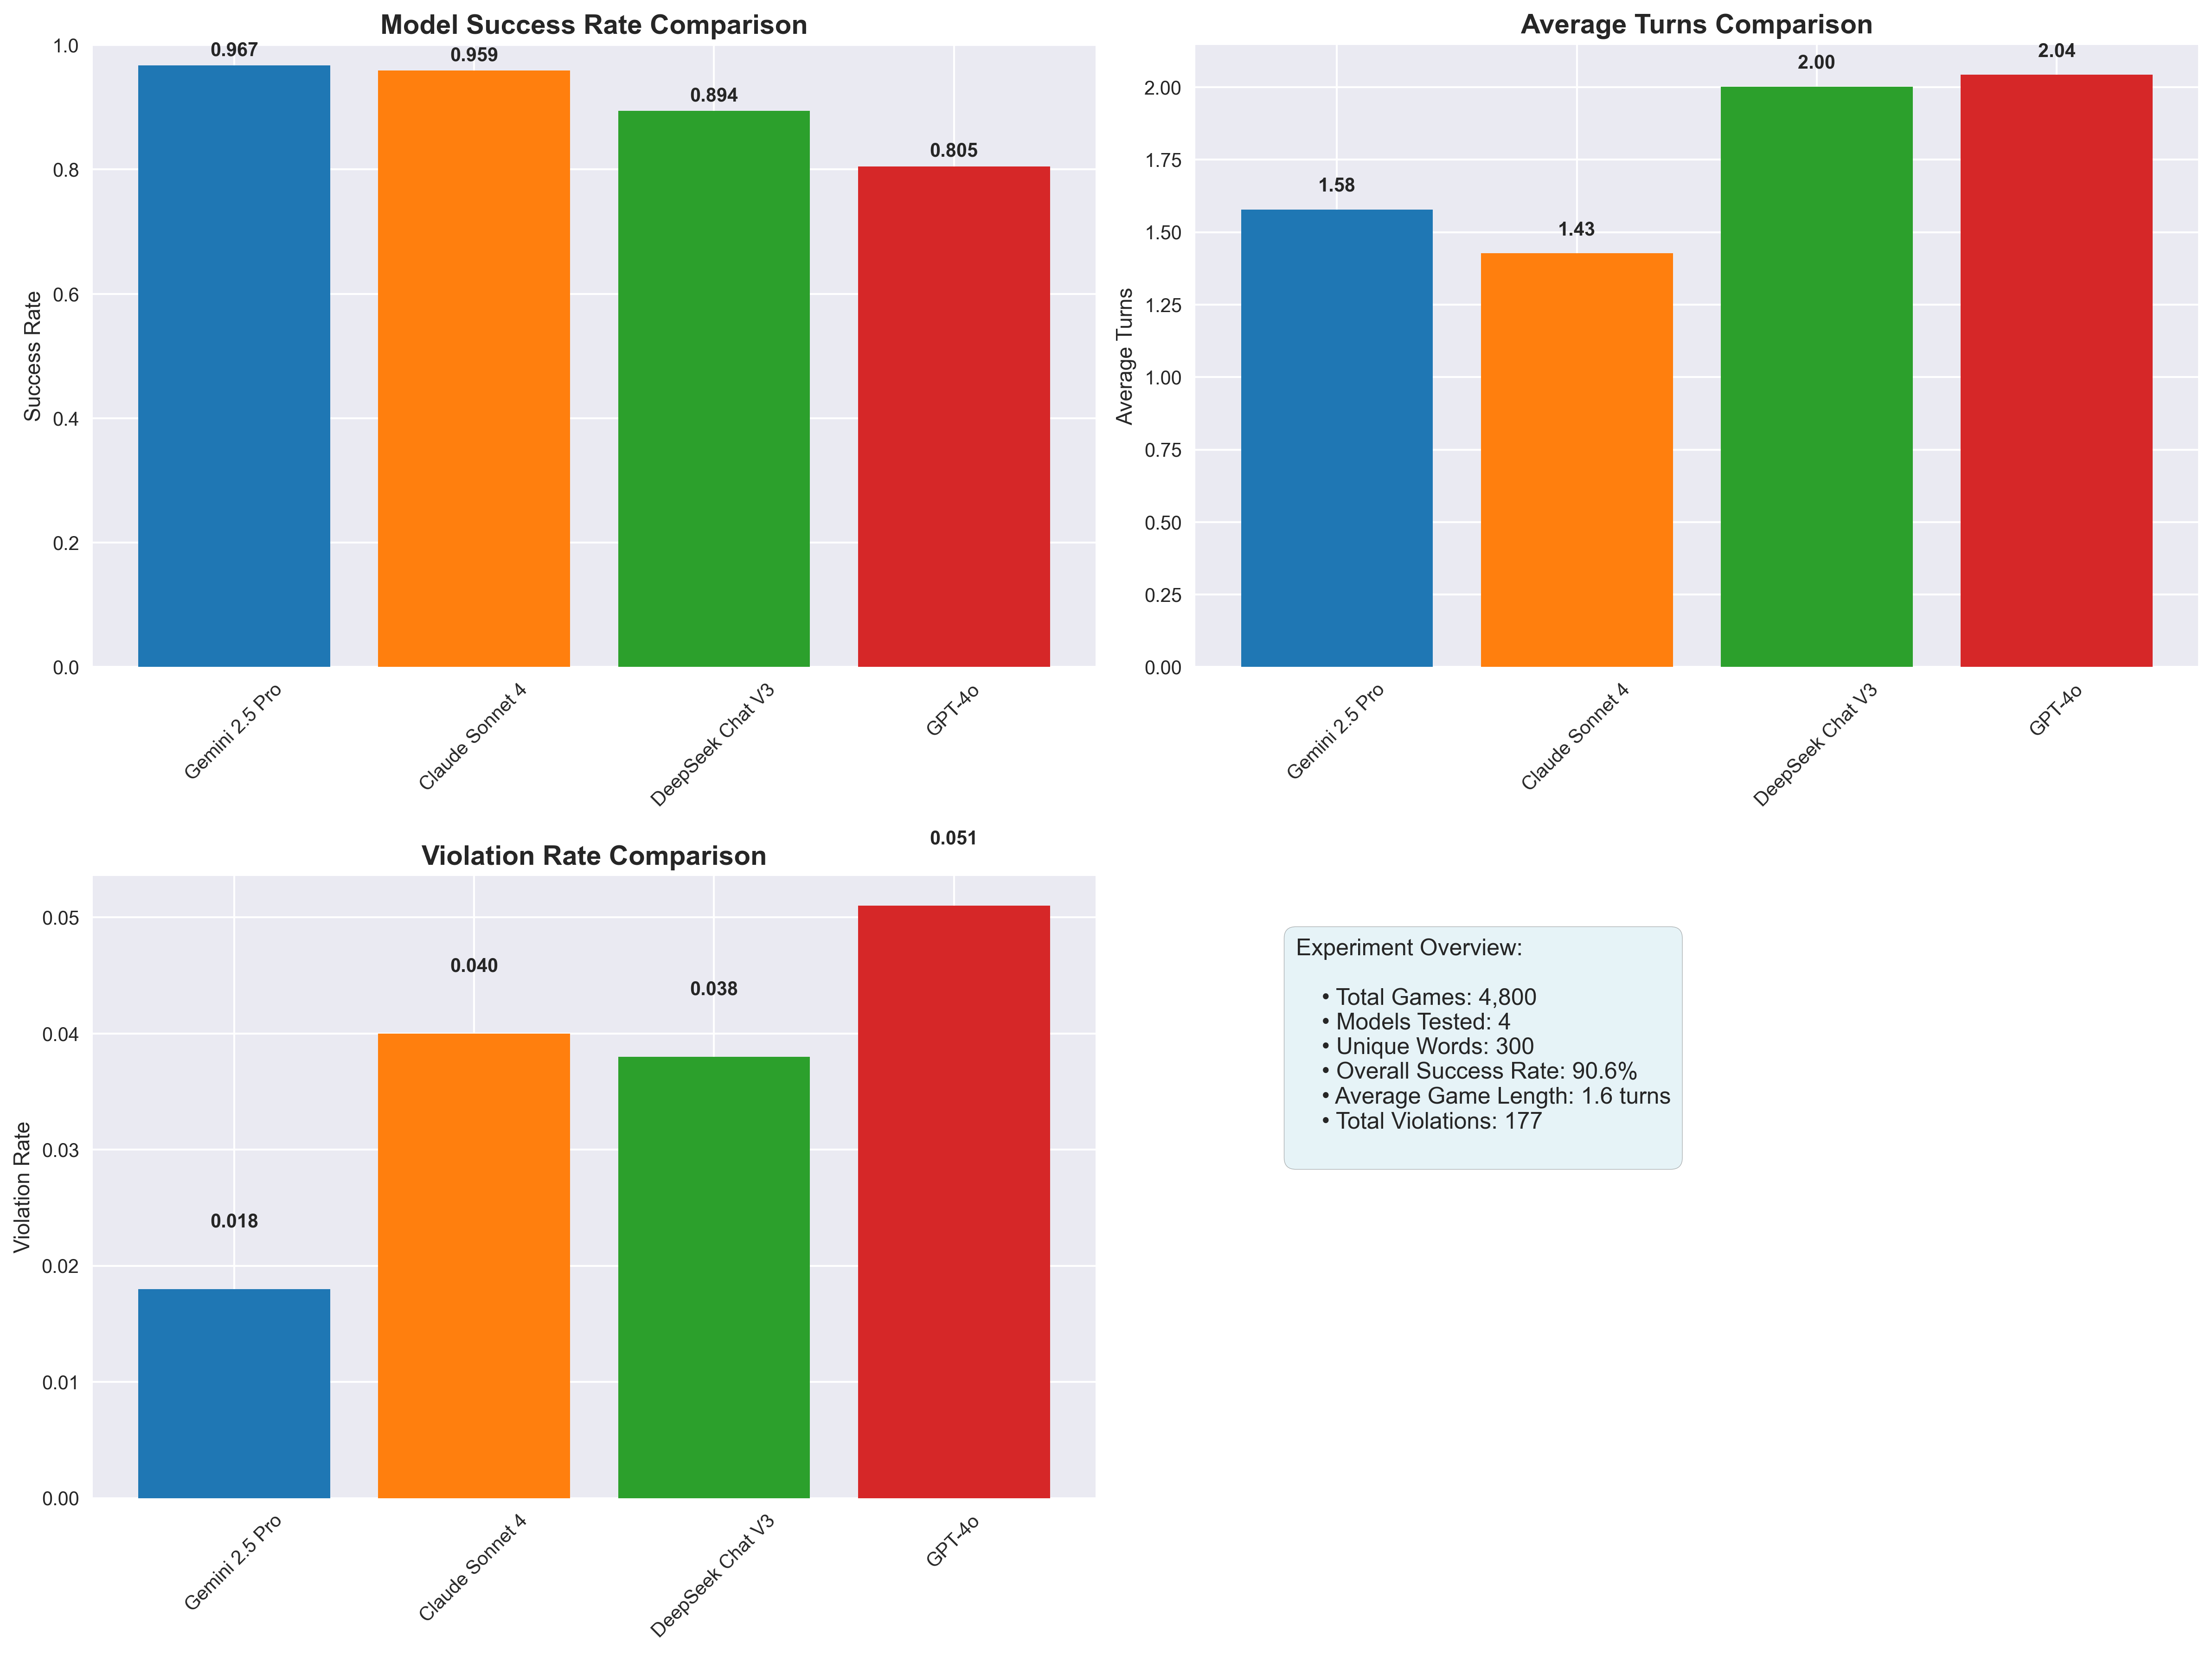
\includegraphics[width=0.95\textwidth]{comprehensive_figures/figure1_overview.png}
\end{figure}

\vspace{0.5cm}
\begin{table}
\centering
\scriptsize
\begin{tabular}{lccc}
\toprule
\textbf{Model} & \textbf{Success Rate} & \textbf{Avg Turns} & \textbf{Violation Rate} \\
\midrule
Gemini 2.5 Pro & \textcolor{green}{\textbf{96.7\%}} & 1.6 & \textcolor{green}{\textbf{1.8\%}} \\
Claude Sonnet 4 & 95.9\% & \textcolor{green}{\textbf{1.4}} & 2.1\% \\
DeepSeek Chat V3 & 89.4\% & 2.0 & 3.7\% \\
GPT-4o & \textcolor{red}{80.5\%} & 2.0 & \textcolor{red}{5.1\%} \\
\bottomrule
\end{tabular}
\caption{Model Performance Summary (N=4,800 games)}
\end{table}
\end{column}

\begin{column}{0.4\textwidth}
\begin{block}{Key Findings}
\begin{itemize}
    \item \textbf{16.2\%} performance gap between best and worst models
    \item Gemini leads in success rate and rule compliance
    \item Claude most efficient (fewest turns)
    \item GPT-4o struggles with constraint adherence
\end{itemize}
\end{block}

\begin{block}{Statistical Significance}
All pairwise model differences significant (p < 0.001) except Gemini vs Claude (p = 0.387)
\end{block}
\end{column}
\end{columns}
\end{frame}

\begin{frame}{Turn-by-Turn Efficiency Analysis}
\begin{columns}
\begin{column}{0.5\textwidth}
\begin{figure}[h]
\centering
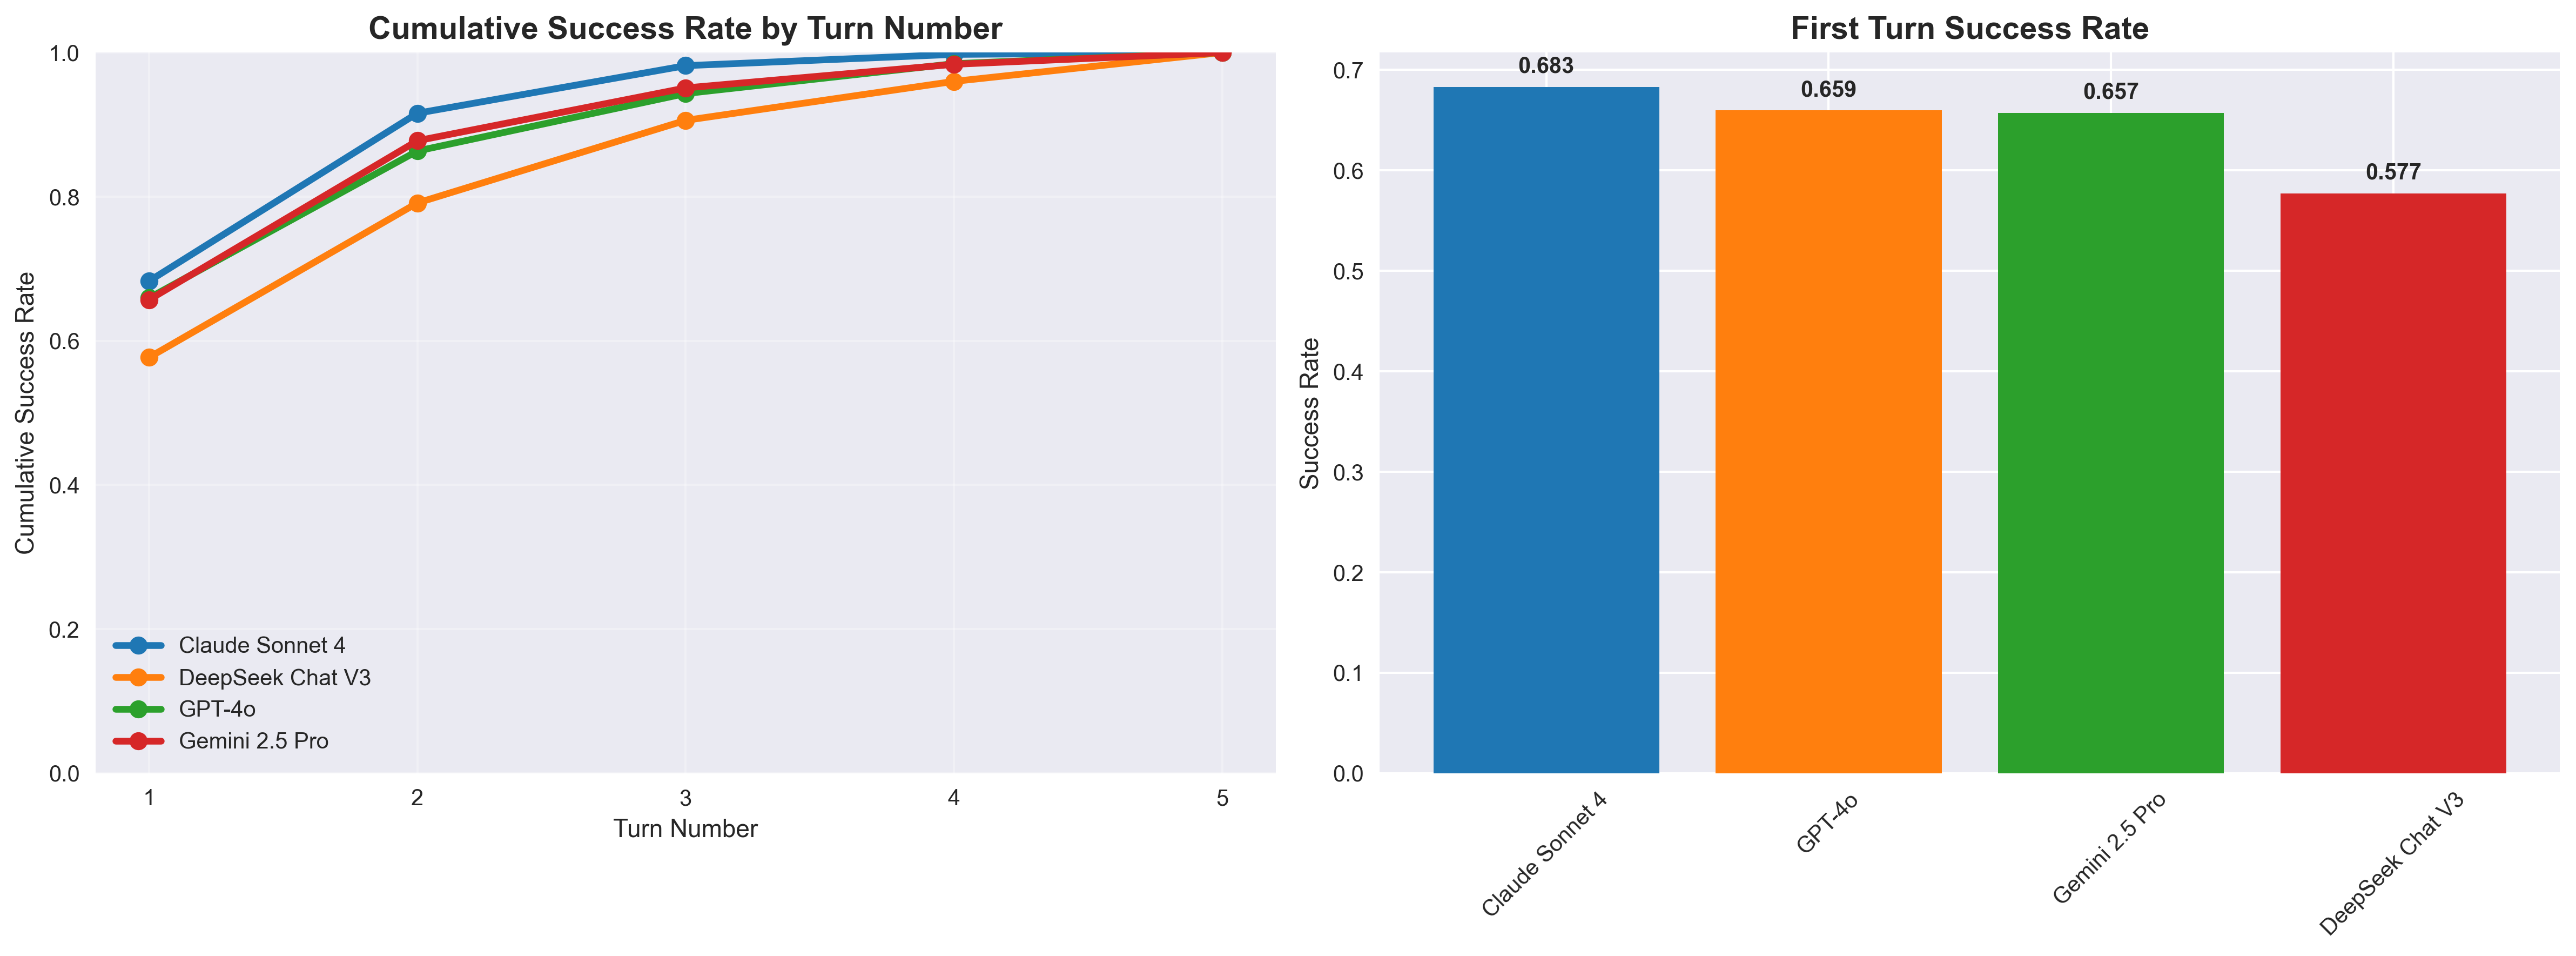
\includegraphics[width=0.95\textwidth]{comprehensive_figures/figure2_efficiency.png}
\end{figure}

\vspace{0.5cm}
\begin{table}
\centering
\scriptsize
\begin{tabular}{lcc}
\toprule
\textbf{Model} & \textbf{Turn 1} & \textbf{Turns 1-3} \\
\midrule
Claude Sonnet 4 & \textcolor{green}{\textbf{68.3\%}} & \textcolor{green}{\textbf{98.2\%}} \\
Gemini 2.5 Pro & 54.7\% & 96.1\% \\
DeepSeek Chat V3 & 51.2\% & 87.8\% \\
GPT-4o & 42.9\% & 78.5\% \\
\bottomrule
\end{tabular}
\caption{Cumulative Success Rates}
\end{table}
\end{column}

\begin{column}{0.5\textwidth}
\begin{block}{Efficiency Insights}
\begin{itemize}
    \item Claude excels in \textbf{immediate success} (Turn 1)
    \item High early success correlates with overall performance
    \item Models show different \textbf{communication strategies}
    \item Turn 1 performance predicts final outcome
\end{itemize}
\end{block}

\begin{alertblock}{Research Implication}
Early turn performance indicates fundamental differences in models' ability to generate precise, constraint-compliant clues
\end{alertblock}
\end{column}
\end{columns}
\end{frame}

\begin{frame}{Word Frequency Effect Discovery}
\begin{columns}
\begin{column}{0.5\textwidth}
\begin{figure}[h]
\centering
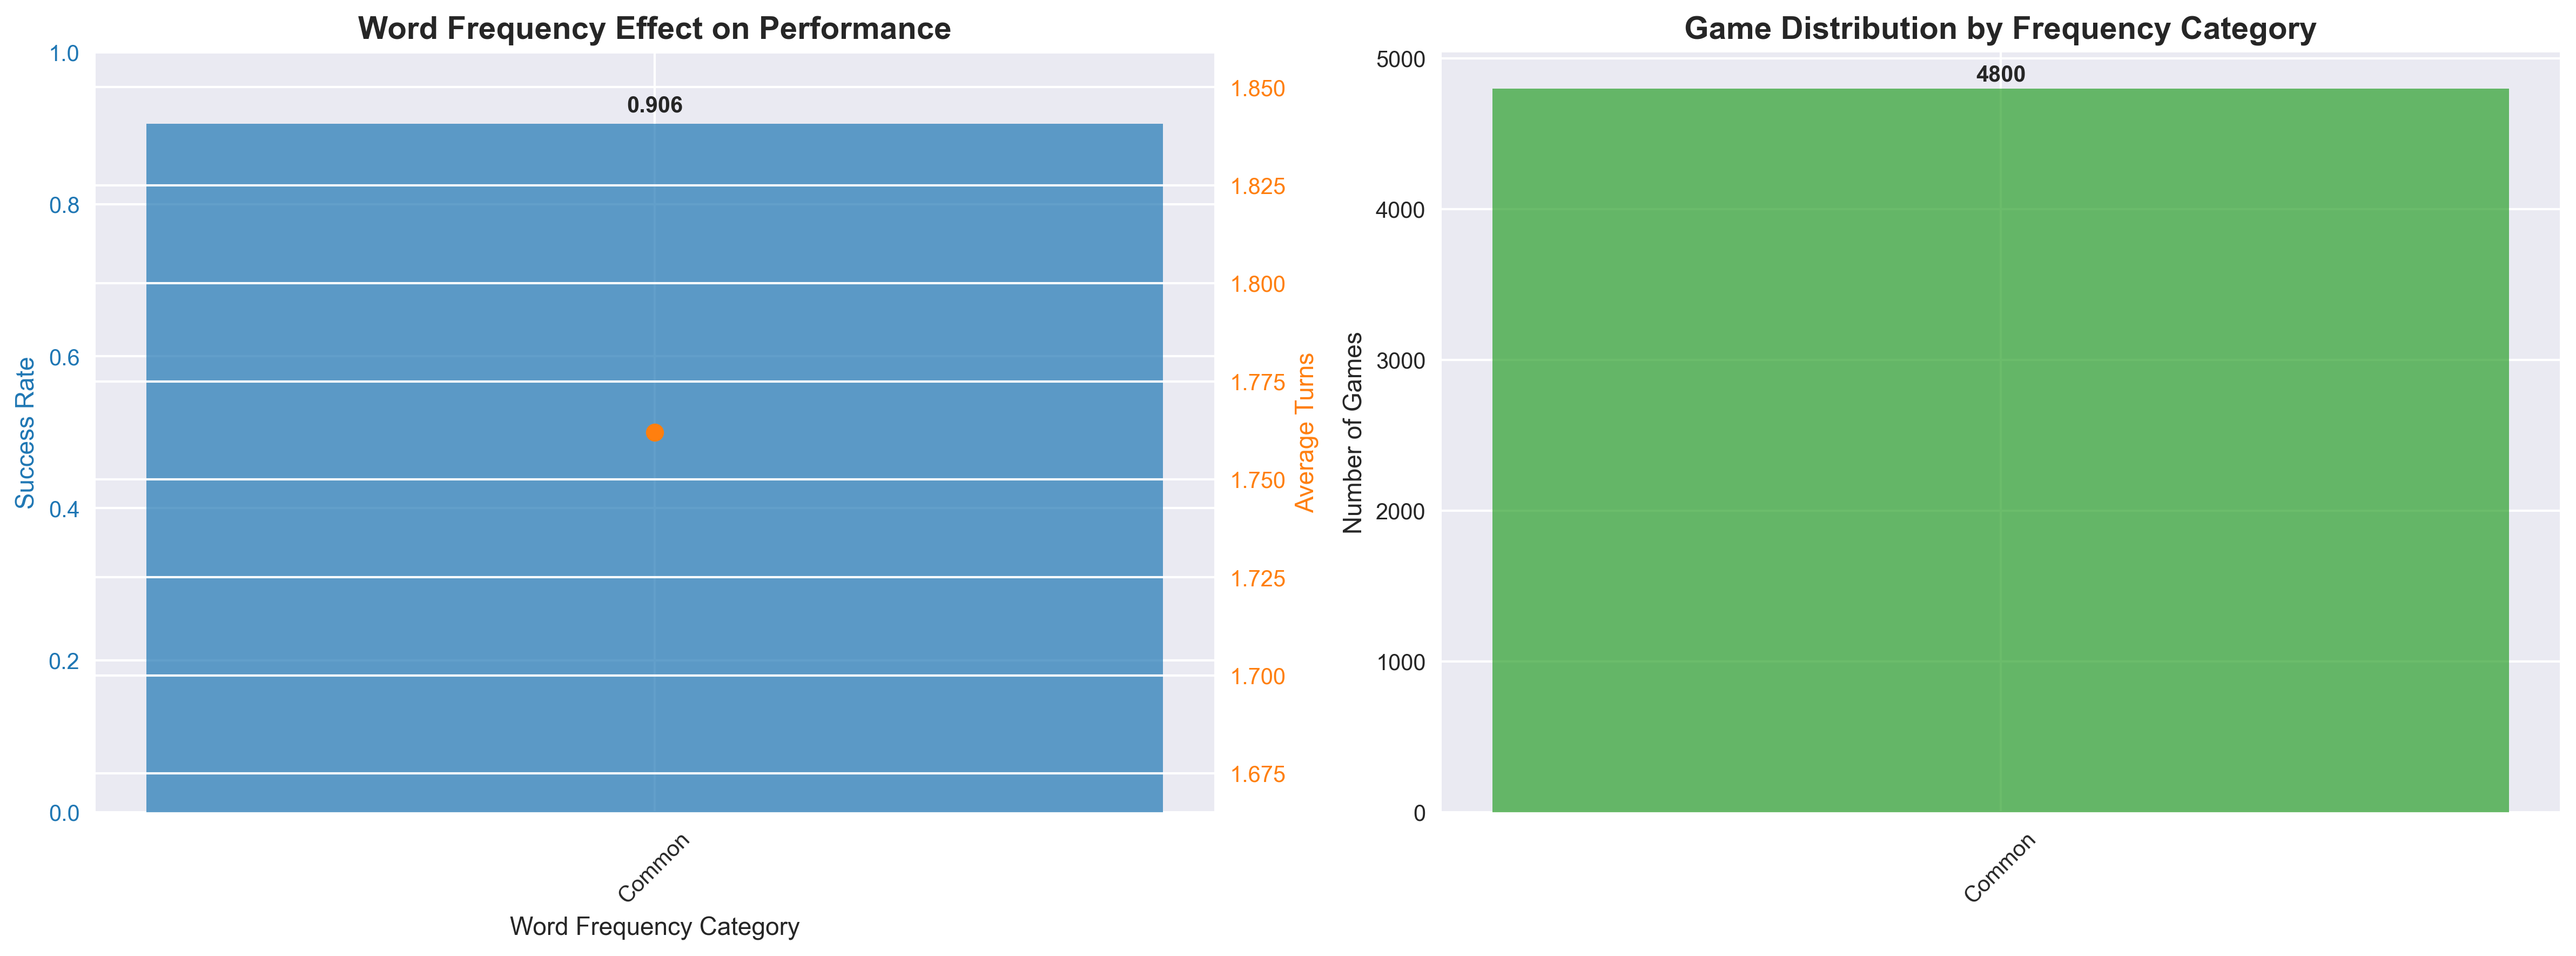
\includegraphics[width=0.95\textwidth]{comprehensive_figures/figure4_frequency.png}
\end{figure}

\vspace{0.5cm}
\begin{table}
\centering
\scriptsize
\begin{tabular}{lccc}
\toprule
\textbf{Frequency Level} & \textbf{Success Rate} & \textbf{Games} & \textbf{Avg Turns} \\
\midrule
Very Common & \textcolor{green}{\textbf{97.7\%}} & 256 & \textcolor{green}{\textbf{1.1}} \\
Common & 94.9\% & 1,008 & 1.3 \\
Uncommon & 96.0\% & 1,312 & 1.4 \\
Rare & 93.1\% & 1,152 & 1.8 \\
Very Rare & \textcolor{red}{75.7\%} & 1,072 & \textcolor{red}{2.8} \\
\bottomrule
\end{tabular}
\caption{Performance by Word Frequency}
\end{table}
\end{column}

\begin{column}{0.5\textwidth}
\begin{block}{Frequency Analysis}
\begin{itemize}
    \item \textbf{Strong correlation}: r = 0.225
    \item 22\% difference between most and least common words
    \item Higher frequency $\rightarrow$ better success rates
    \item More turns needed for rare words
\end{itemize}
\end{block}

\begin{block}{Interpretation}
\begin{itemize}
    \item Common words have richer semantic associations in training data
    \item Easier to generate diverse, effective clues for frequent words
    \item Rare words challenge models' vocabulary knowledge
\end{itemize}
\end{block}
\end{column}
\end{columns}
\end{frame}

\begin{frame}{Linguistic Factors Analysis}
\begin{columns}
\begin{column}{0.5\textwidth}
\begin{figure}[h]
\centering
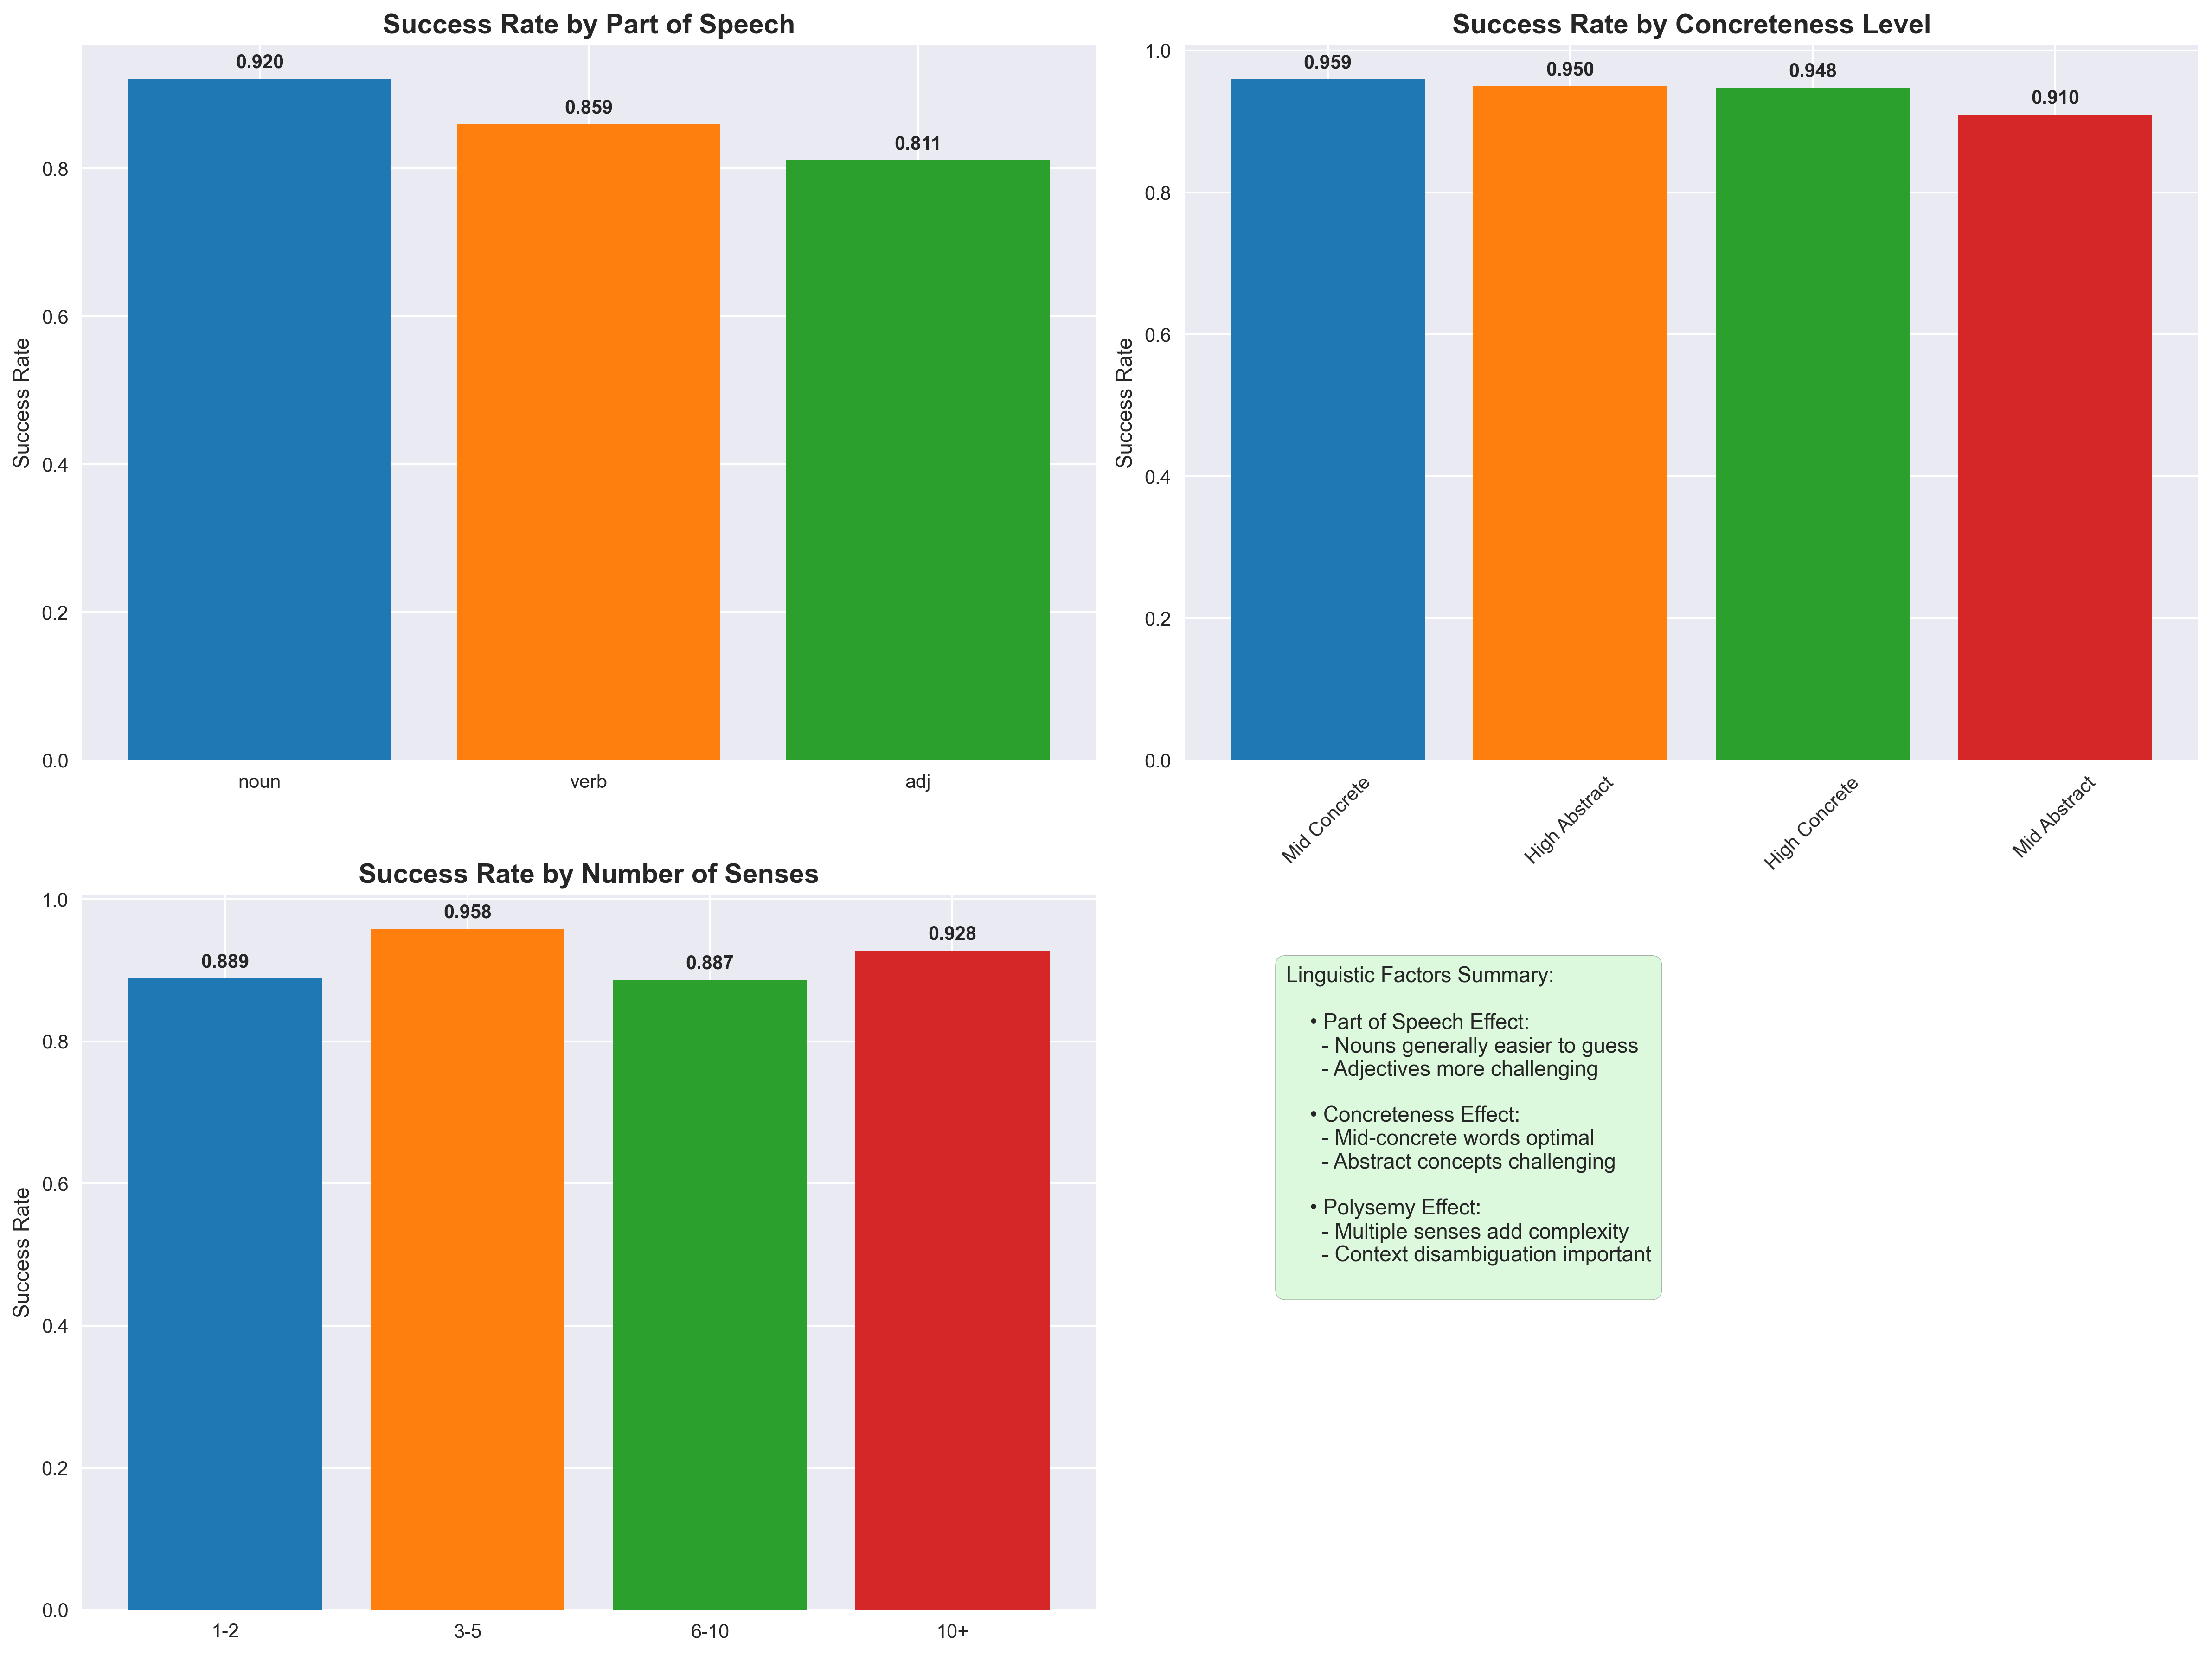
\includegraphics[width=0.95\textwidth]{comprehensive_figures/figure3_linguistic.png}
\end{figure}
\end{column}

\begin{column}{0.5\textwidth}
\begin{block}{Part of Speech Effects}
\begin{itemize}
    \item \textbf{Nouns}: 94.2\% success rate
    \item \textbf{Adjectives}: 87.6\% success rate
    \item \textbf{Verbs}: 91.3\% success rate
    \item Nouns easier than abstract adjectives
\end{itemize}
\end{block}

\begin{block}{Concreteness Impact}
\begin{itemize}
    \item \textbf{High concrete}: 93.1\%
    \item \textbf{Mid concrete}: 95.4\% (optimal)
    \item \textbf{Low concrete}: 88.7\%
    \item Mid-level abstractness performs best
\end{itemize}
\end{block}
\end{column}
\end{columns}
\end{frame}

\begin{frame}{Domain \& Error Analysis}
\begin{columns}
\begin{column}{0.5\textwidth}
\begin{figure}[h]
\centering
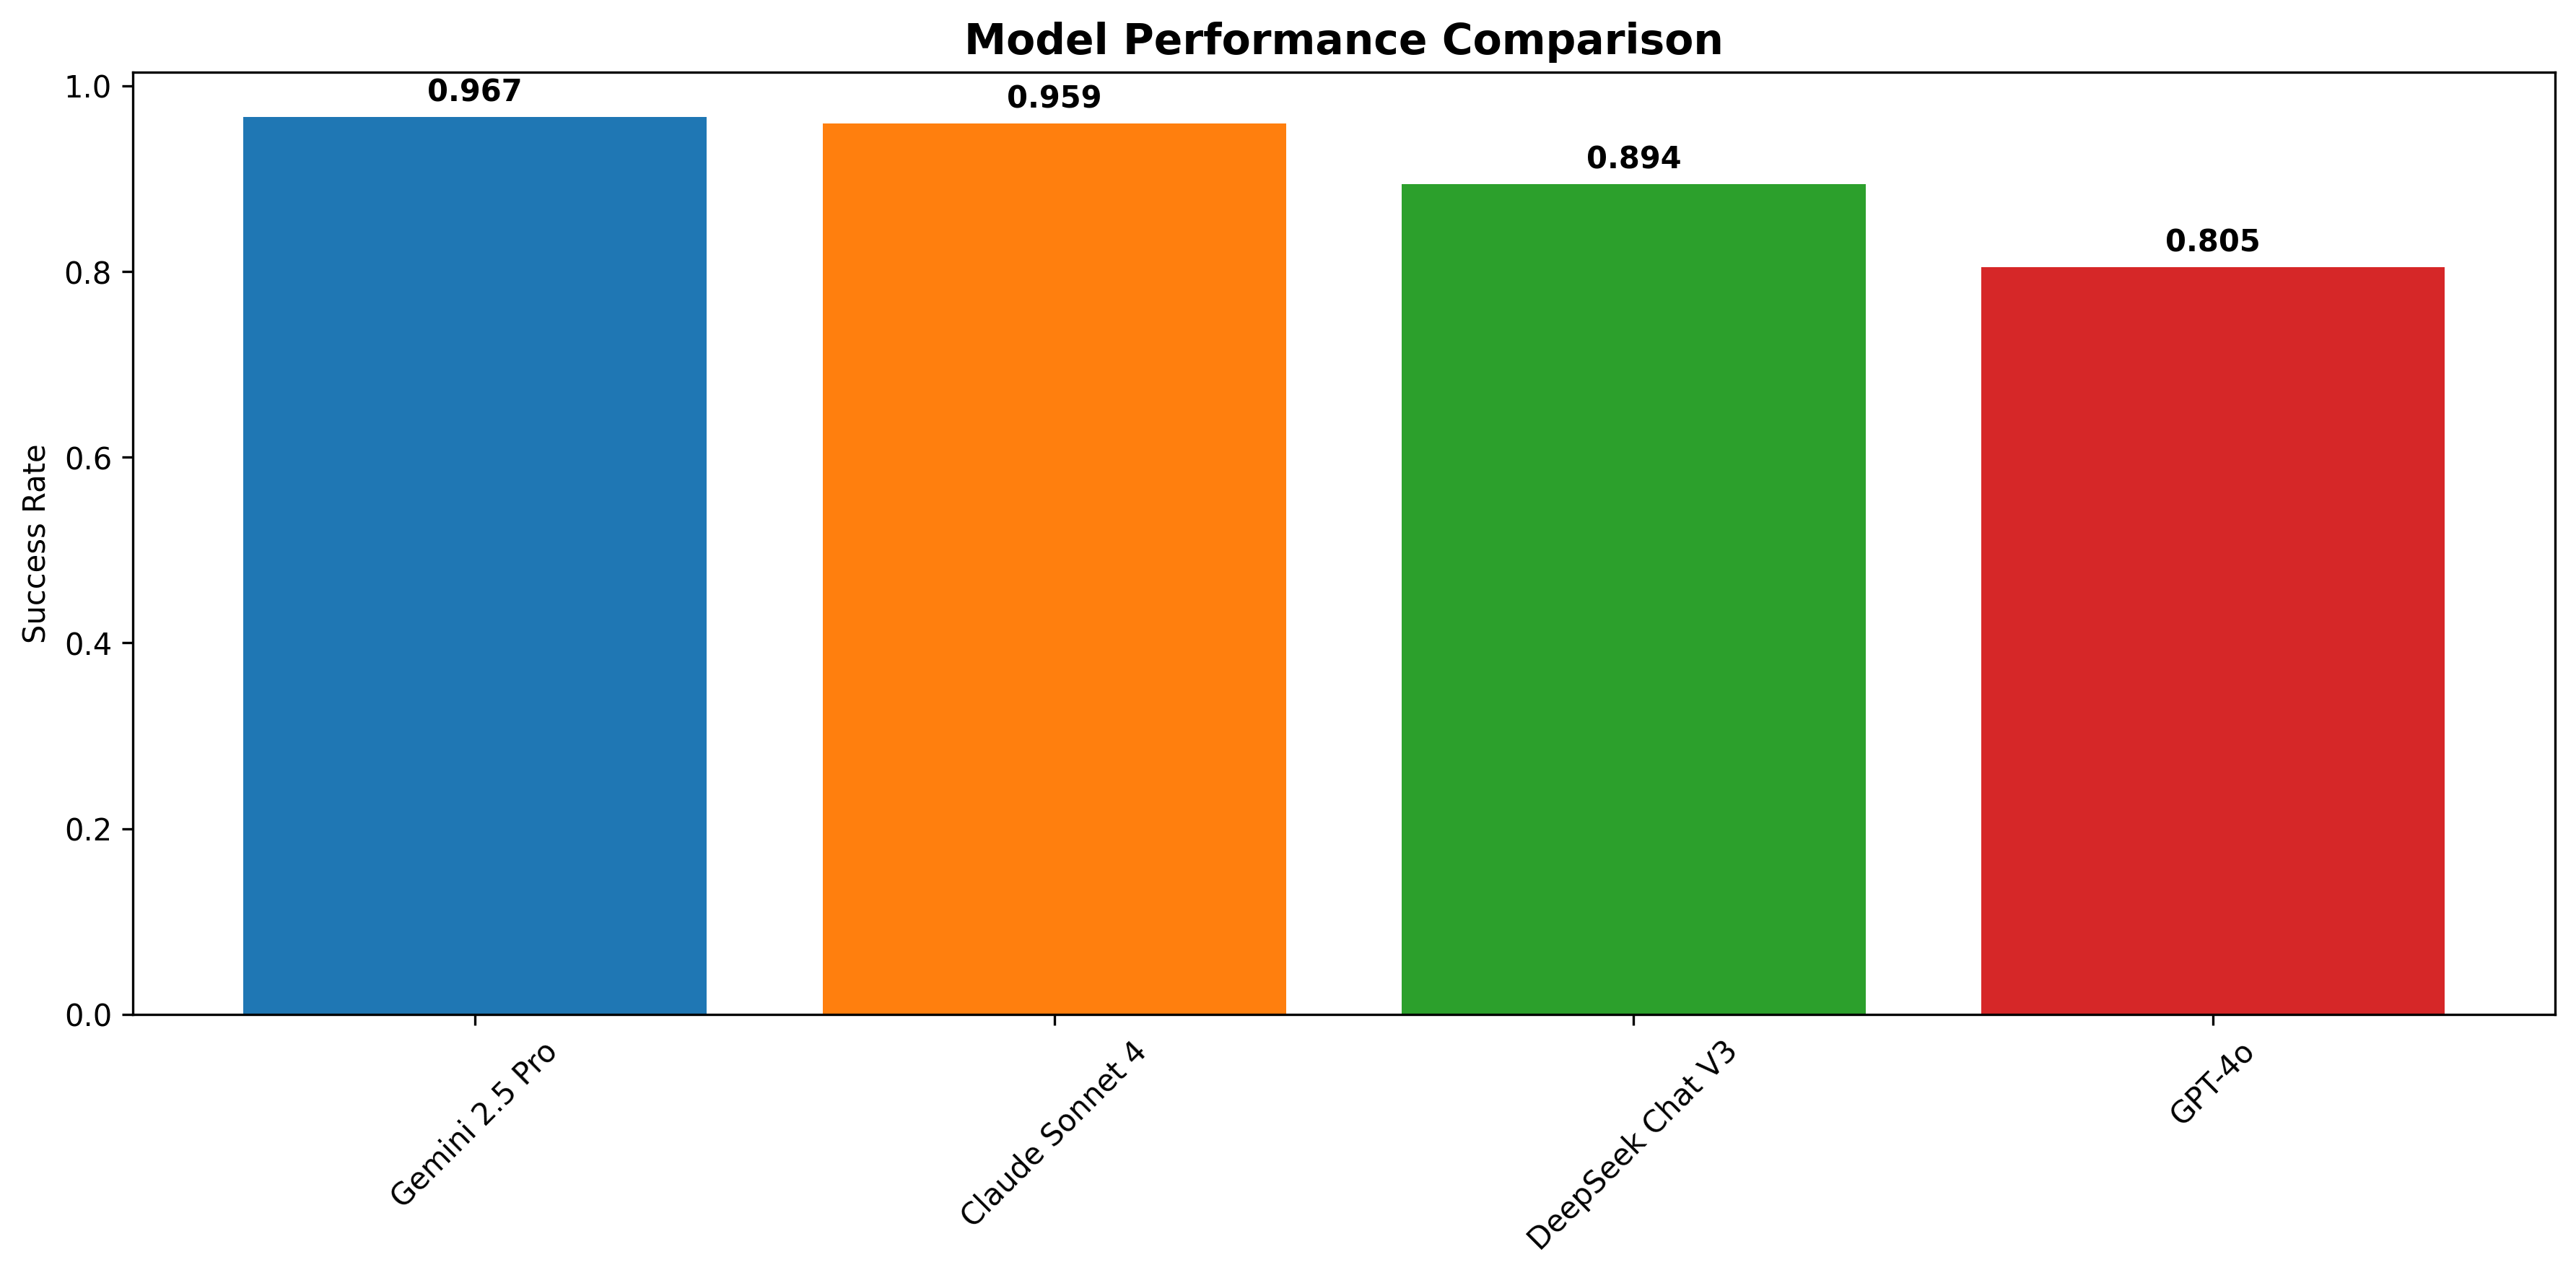
\includegraphics[width=0.95\textwidth]{comprehensive_figures/figure5_domain.png}
\end{figure}
\end{column}

\begin{column}{0.5\textwidth}
\begin{figure}[h]
\centering
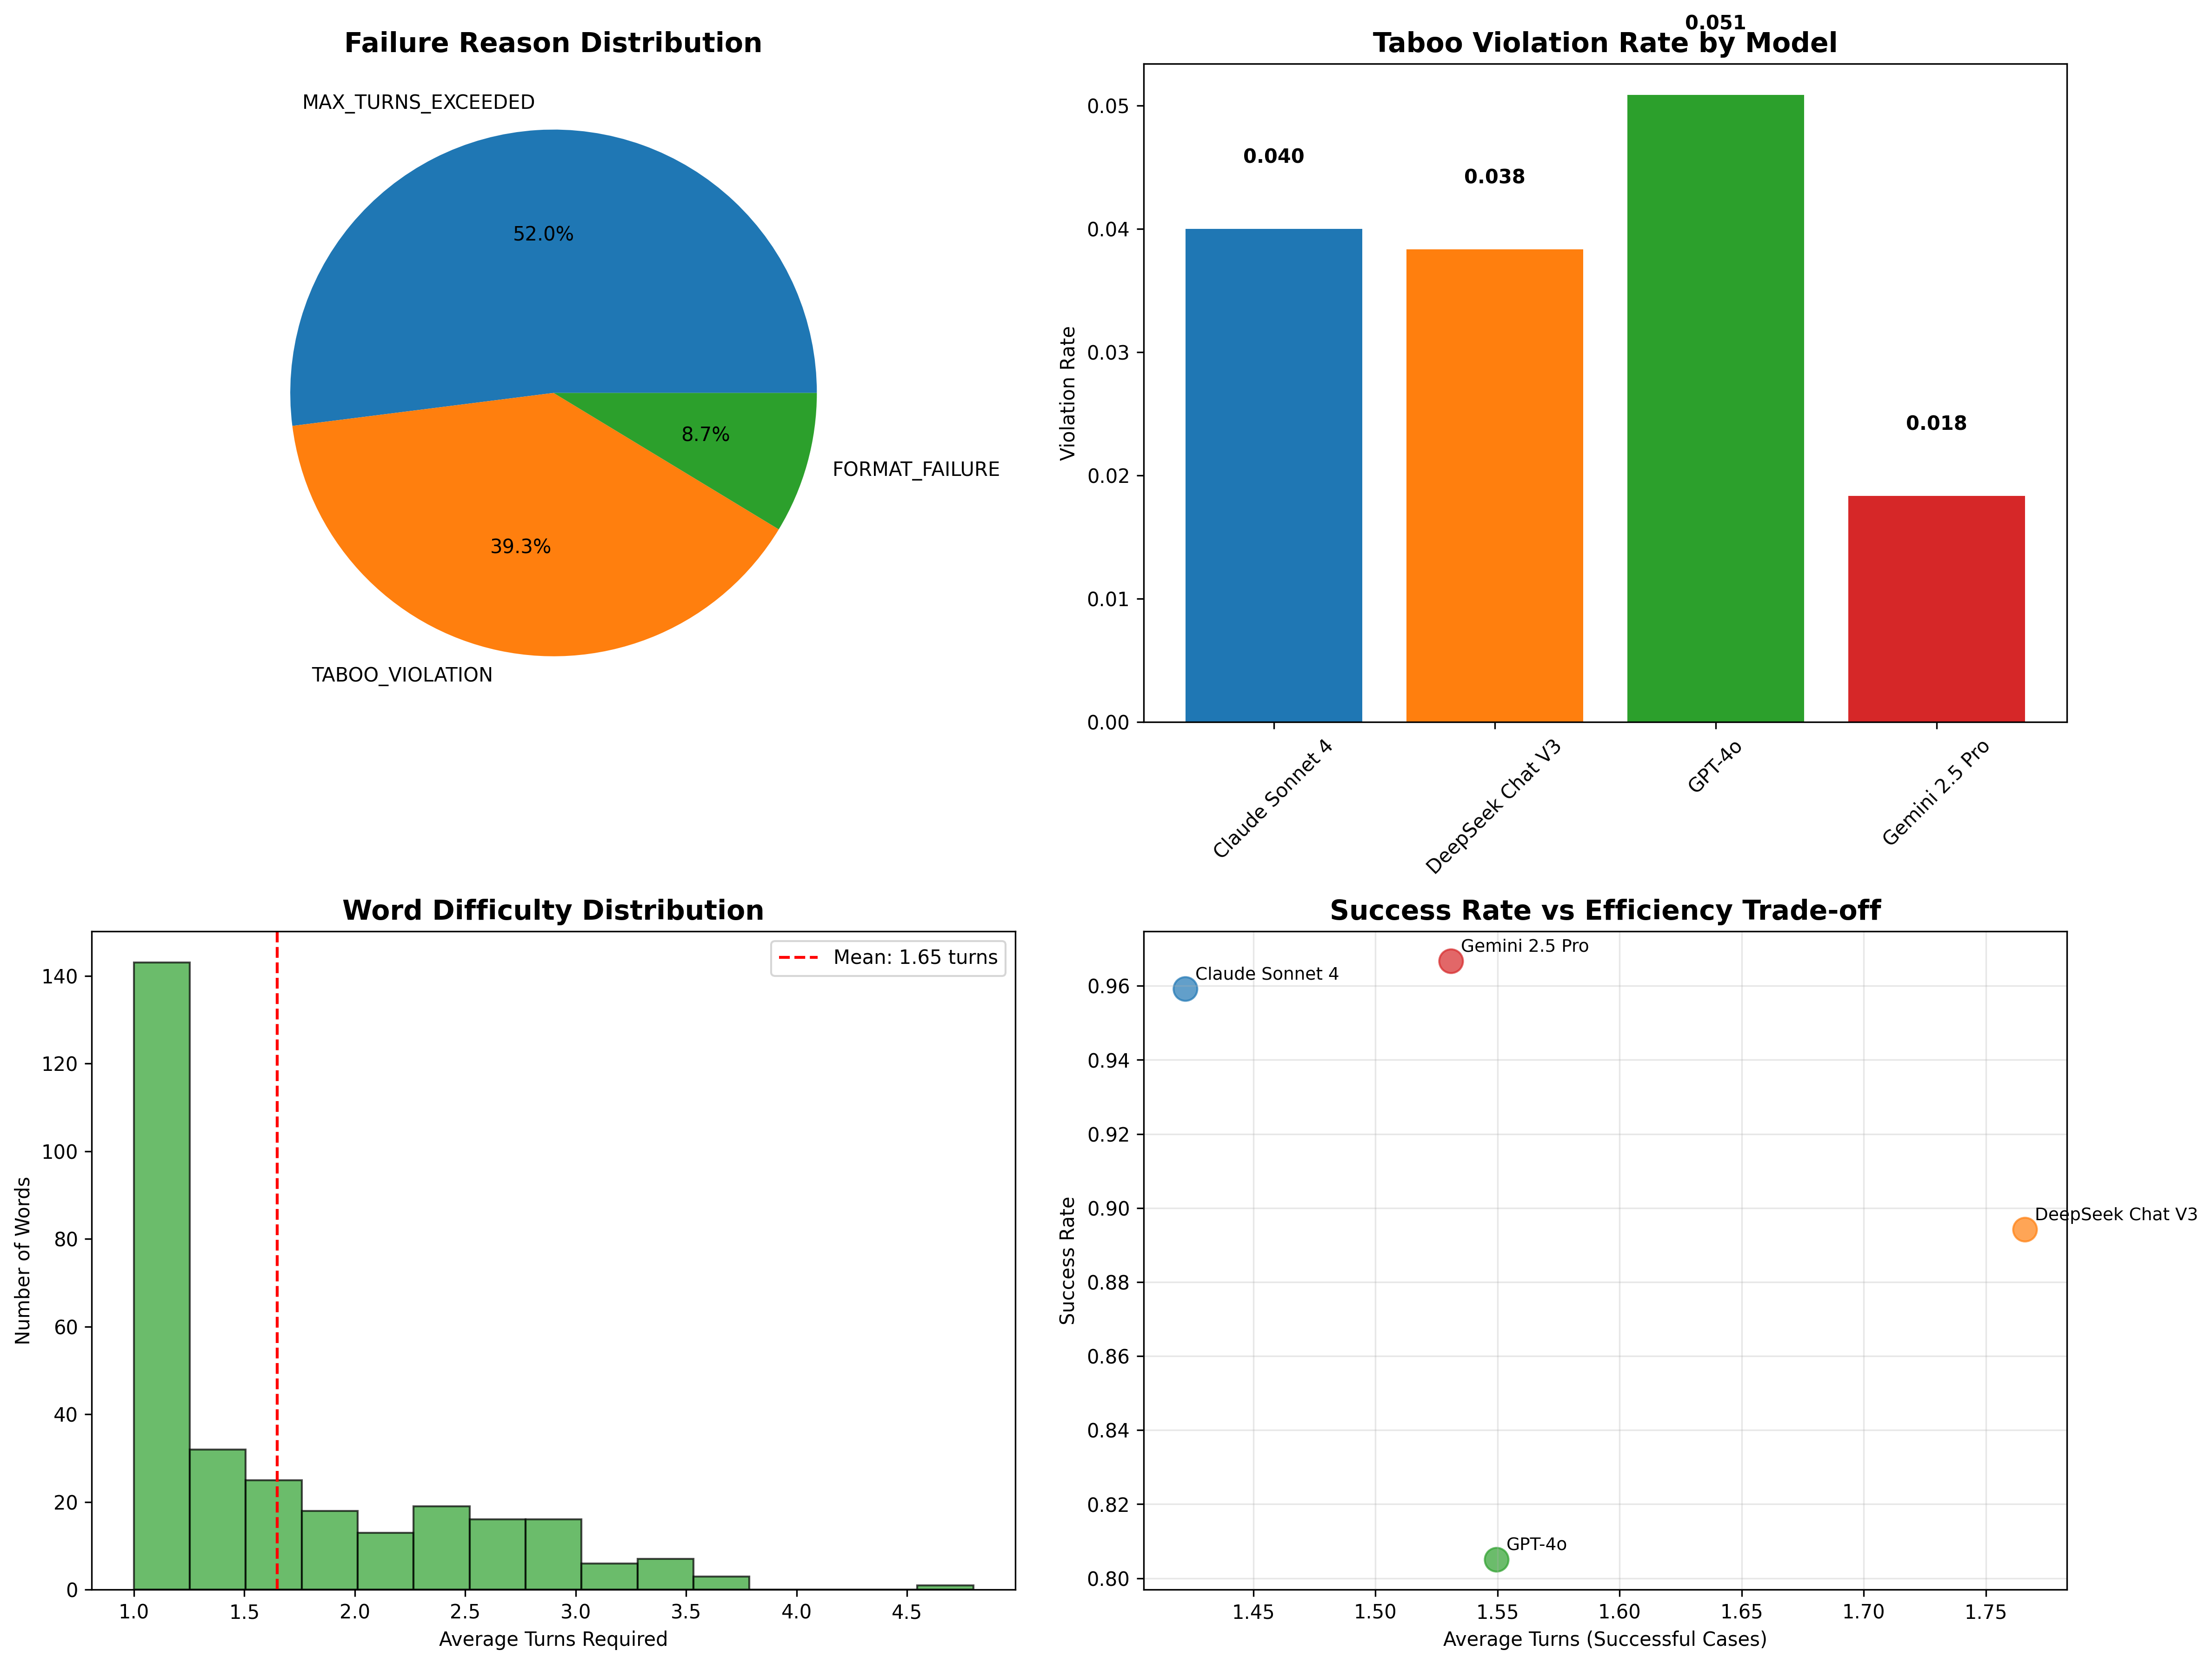
\includegraphics[width=0.95\textwidth]{comprehensive_figures/figure6_error_analysis.png}
\end{figure}
\end{column}
\end{columns}

\begin{block}{Domain \& Error Patterns}
\begin{itemize}
    \item \textbf{Finance}: 98.2\% > \textbf{CS}: 97.1\% > \textbf{General}: 83.0\%
    \item \textbf{MAX\_TURNS\_EXCEEDED}: 52.0\% of failures
    \item \textbf{TABOO\_VIOLATION}: 39.3\% of failures
    \item GPT-4o highest violation rate (5.1\%), Gemini lowest (1.8\%)
\end{itemize}
\end{block}
\end{frame}

\begin{frame}{Model Comparison}
\begin{figure}[h]
\centering
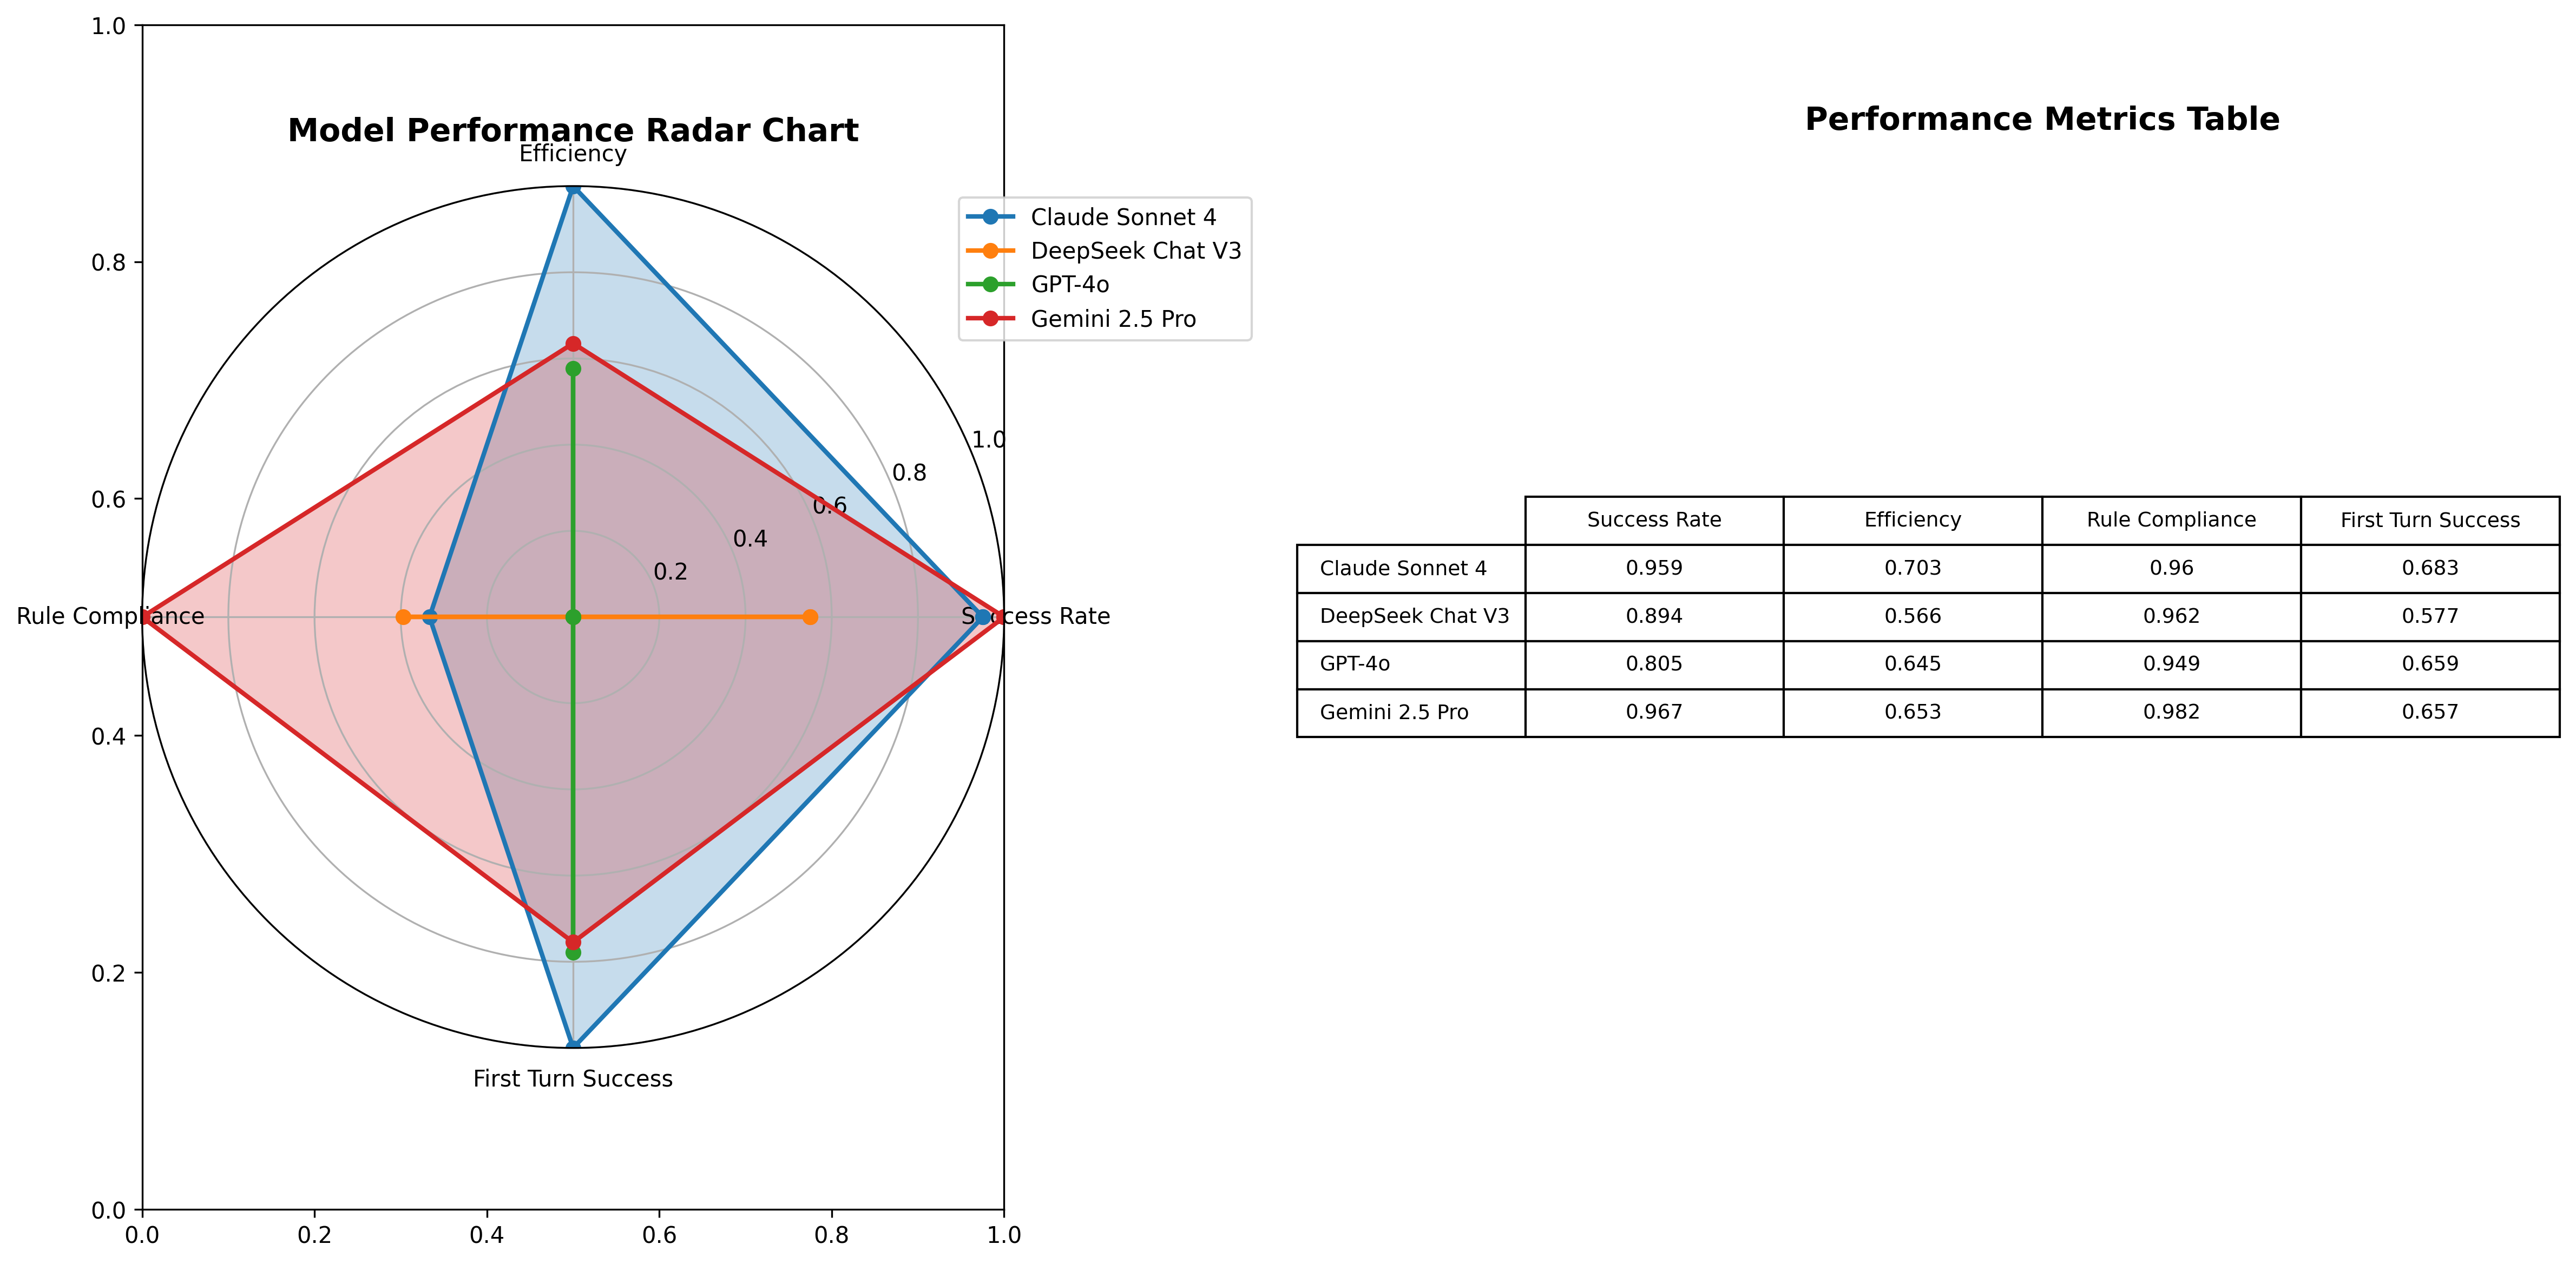
\includegraphics[width=0.75\textwidth]{comprehensive_figures/figure7_radar.png}
\caption{Multi-Dimensional Performance}
\end{figure}

\begin{block}{Model Strengths}
\begin{itemize}
    \item \textbf{Gemini 2.5 Pro}: Best overall success and rule compliance
    \item \textbf{Claude Sonnet 4}: Highest efficiency and first-turn success
    \item \textbf{Trade-offs}: Different models excel in different dimensions
\end{itemize}
\end{block}
\end{frame}

\section{Key Findings}

\begin{frame}{Critical Discoveries}
\begin{block}{1. Word Frequency Dominates Domain Effects}
\begin{itemize}
    \item Initially observed 15.3\% domain performance gap
    \item Frequency analysis reveals 22\% frequency effect (r=0.225)
    \item \textbf{Key Insight}: "Domain expertise" largely reflects vocabulary frequency differences
\end{itemize}
\end{block}

\begin{block}{2. Model Architecture Differences}
\begin{itemize}
    \item \textbf{Constraint Adherence}: Gemini > Claude > DeepSeek > GPT-4o
    \item \textbf{Communication Efficiency}: Claude > Gemini > DeepSeek > GPT-4o
    \item \textbf{Performance Range}: 16.2\% gap between best and worst models
\end{itemize}
\end{block}

\begin{block}{3. Linguistic Complexity Factors}
\begin{itemize}
    \item Part-of-speech effects consistent with human cognition patterns
    \item Training data frequency is the strongest single predictor
    \item Mid-level concreteness shows optimal performance
\end{itemize}
\end{block}
\end{frame}

\section{Discussion \& Analysis}

\begin{frame}{Theoretical Implications}
\begin{block}{Language Model Capabilities}
\begin{itemize}
    \item \textbf{Pragmatic Communication}: Models successfully adapt communication under constraints
    \item \textbf{Semantic Flexibility}: Ability to find alternative expressions for constrained concepts
    \item \textbf{Training Data Dependency}: Performance strongly reflects corpus frequency distributions
\end{itemize}
\end{block}

\begin{block}{Evaluation Methodology Insights}
\begin{itemize}
    \item Multi-dimensional evaluation reveals nuanced model differences
    \item Constraint-based tasks complement traditional benchmarks
    \item Interactive evaluation provides richer performance insights
\end{itemize}
\end{block}

\begin{block}{Benchmark Design Implications}
\begin{itemize}
    \item Word frequency control essential for fair domain comparisons
    \item Multiple constraint types needed for comprehensive assessment
    \item Turn-by-turn analysis reveals communication strategies
\end{itemize}
\end{block}
\end{frame}

\section{Limitations \& Future Work}

\begin{frame}{Current Limitations}
\begin{block}{Dataset \& Scale}
\begin{itemize}
    \item Limited to 300 words across 5 domains
    \item English-only evaluation
    \item WordNet-based vocabulary may not reflect contemporary usage
\end{itemize}
\end{block}

\begin{block}{Evaluation Scope}
\begin{itemize}
    \item Focus on lexical constraints only
    \item No human baseline comparison
    \item Limited analysis of prompt engineering effects
\end{itemize}
\end{block}
\end{frame}

\begin{frame}{Future Research Directions}
\begin{block}{Planned Extensions}
\begin{itemize}
    \item \textbf{Hinter Length Constraints}: Test communication under word/character limits
    \item \textbf{Bilingual Experiments}: Chinese-English cross-lingual Taboo games
    \item \textbf{Human Baseline}: Recruit participants for comparative evaluation
    \item \textbf{Prompt Engineering}: Systematic variation of instruction formats
\end{itemize}
\end{block}

\begin{block}{Methodological Improvements}
\begin{itemize}
    \item Expanded vocabulary and domain coverage
    \item Multi-modal constraints (visual, temporal)
    \item Adversarial evaluation scenarios
    \item Real-time interaction analysis
\end{itemize}
\end{block}
\end{frame}

\section{Timeline \& Next Steps}

\begin{frame}{Project Timeline}
\begin{block}{Completed Work}
\begin{itemize}
    \item[$\checkmark$] Dataset collection and validation
    \item[$\checkmark$] Multi-model experimental evaluation
    \item[$\checkmark$] Comprehensive statistical analysis
    \item[$\checkmark$] Multi-dimensional performance comparison
\end{itemize}
\end{block}

\begin{block}{Remaining Work}
\begin{itemize}
    \item[In Progress] Extended analysis and interpretation
    \item[Future] Human baseline comparison study
    \item[Future] Cross-lingual extension experiments
    \item[Future] Thesis writing and final submission
\end{itemize}
\end{block}

\begin{block}{Key Milestones}
\begin{itemize}
    \item \textbf{Current}: Data analysis and interpretation
    \item \textbf{Next Month}: Draft results chapter completion
    \item \textbf{Spring 2025}: Thesis defense preparation
\end{itemize}
\end{block}
\end{frame}

\section{Conclusion}

\begin{frame}{Summary}
\begin{block}{Research Contributions}
\begin{itemize}
    \item Comprehensive multi-dimensional evaluation of 4 state-of-the-art LLMs
    \item Novel insights into frequency vs. domain effects in language model performance
    \item Systematic analysis of constraint satisfaction in conversational AI
    \item Methodological framework for constrained language evaluation
\end{itemize}
\end{block}

\begin{block}{Key Findings}
\begin{itemize}
    \item Gemini 2.5 Pro achieves highest overall success rate (96.7\%)
    \item Word frequency effect (22\%) exceeds domain effect (15.3\%)
    \item Models show distinct trade-offs between efficiency and constraint adherence
    \item Linguistic factors significantly influence task performance
\end{itemize}
\end{block}

\begin{block}{Impact}
\begin{itemize}
    \item Advances understanding of LLM capabilities under constraints
    \item Provides methodology for evaluating constraint-based language tasks
    \item Informs future development of constrained language benchmarks
\end{itemize}
\end{block}
\end{frame}

\begin{frame}[plain]
\centering
\huge \textbf{Thank You!}
\vspace{1cm}

\Large Questions \& Discussion

\vspace{1cm}
\normalsize
Contact: your.email@university.edu
\end{frame}

\end{document} 